\chapter{Experimental Results \& Model Comparison}

\section{Supervised Classifier Performance Benchmark}
Table~\ref{tab:results_benchmark} documents the hold-out test set performance ($N_{test}=1,800$) across all six benchmarked classification models.

\begin{table}[H]
\centering
\caption{Supervised Classification Benchmark Results (Hold-out Test Set, $N=1,800$)}
\label{tab:results_benchmark}
\small
\begin{tabular}{lcccccc}
\toprule
\textbf{Model Algorithm} & \textbf{Accuracy} & \textbf{Precision} & \textbf{Recall} & \textbf{F1 (Weighted)} & \textbf{ROC-AUC} & \textbf{5-Fold CV Score (F1)} \\
\midrule
Zero-R Baseline & 0.6972 & 0.0000 & 0.0000 & 0.5728 & 0.5000 & $0.5725 \pm 0.0004$ \\
K-Nearest Neighbors & 0.8317 & 0.8201 & 0.5688 & 0.8217 & 0.8678 & $0.8069 \pm 0.0037$ \\
Decision Tree & 0.8644 & 0.8265 & 0.6991 & 0.8610 & 0.9097 & $0.8561 \pm 0.0085$ \\
Naive Bayes & 0.8611 & 0.7496 & 0.8128 & 0.8626 & 0.9271 & $0.8513 \pm 0.0120$ \\
Random Forest & 0.8822 & 0.8612 & 0.7284 & 0.8792 & 0.9361 & $0.8757 \pm 0.0051$ \\
\textbf{Support Vector Machine} & \textbf{0.8917} & \textbf{0.8601} & \textbf{0.7670} & \textbf{0.8898} & \textbf{0.9422} & $\mathbf{0.8954 \pm 0.0047}$ \\
\bottomrule
\end{tabular}
\end{table}

\section{ROC Curves \& Receiver Discrimination}
Figure~\ref{fig:results_roc} depicts ROC curves across all six algorithms. Support Vector Machine (SVC RBF) achieves leading discrimination with an ROC-AUC of $0.9422$, followed by Random Forest ($0.9361$) and Naive Bayes ($0.9271$).

\begin{figure}[H]
\centering
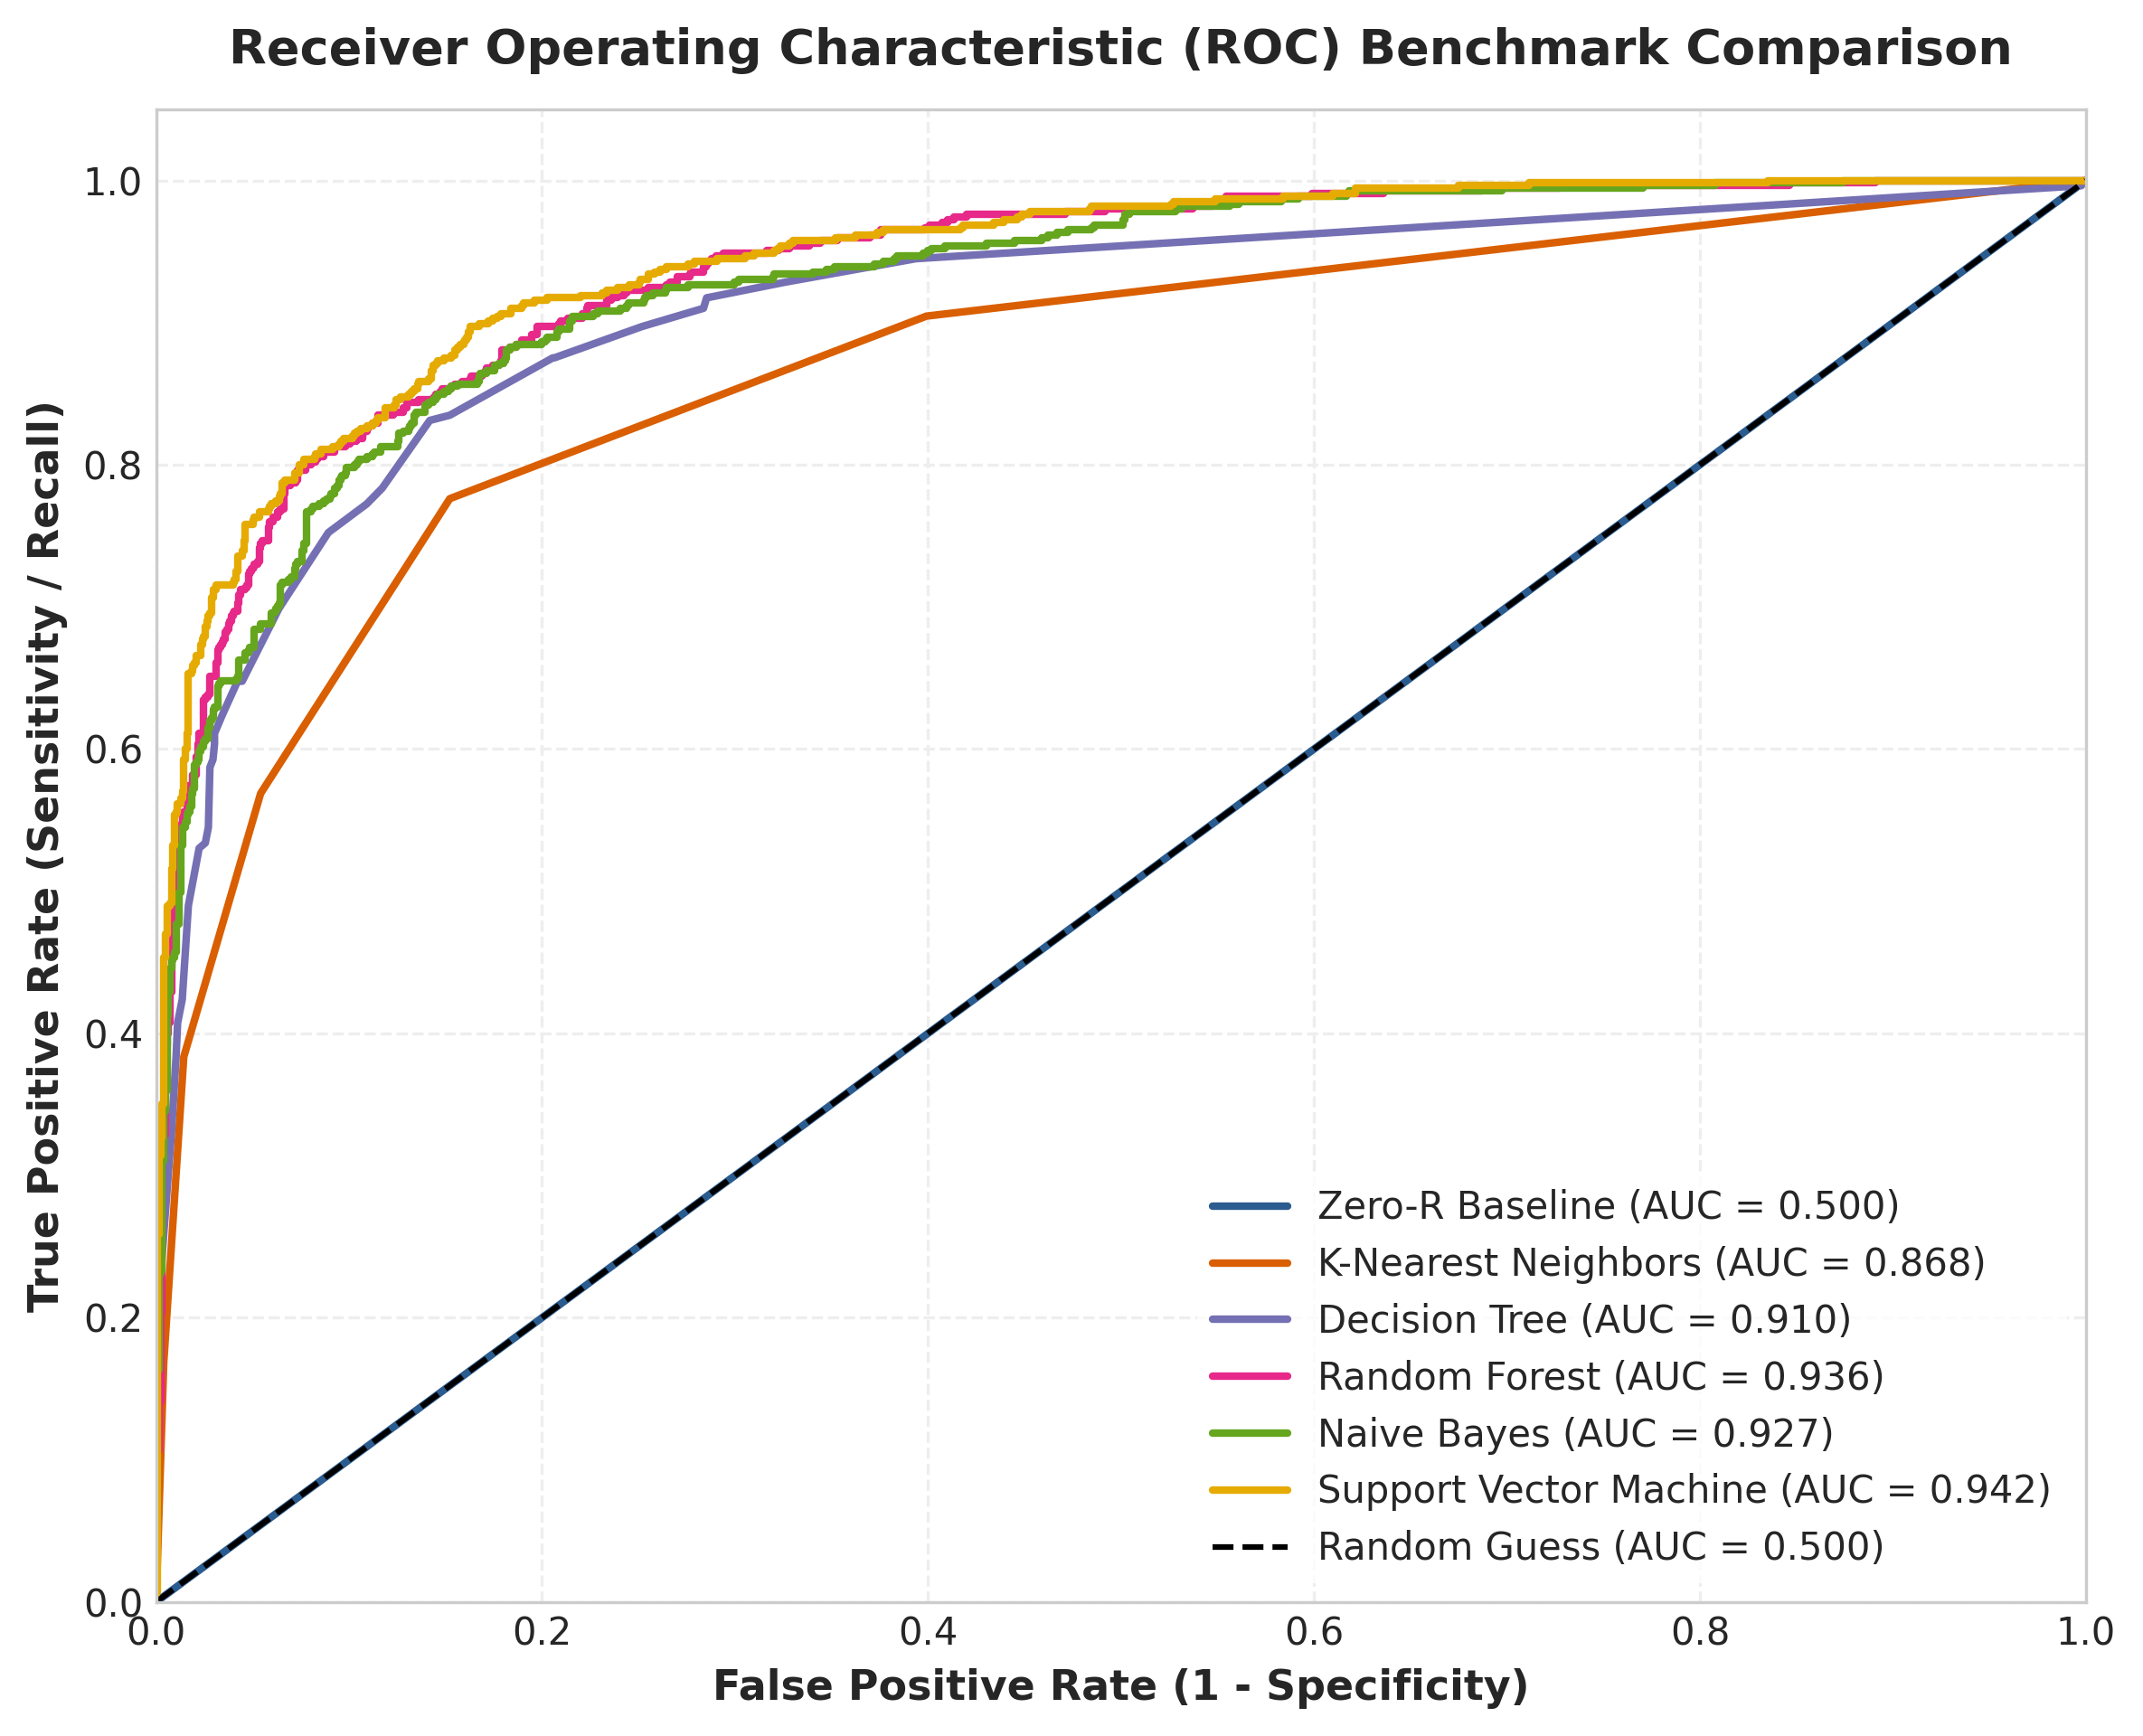
\includegraphics[width=0.75\textwidth]{figures/roc_curves.png}
\caption{Receiver Operating Characteristic (ROC) Benchmark Comparison.}
\label{fig:results_roc}
\end{figure}

\section{Confusion Matrix Analysis}
Figure~\ref{fig:results_cm} presents the confusion matrices on the 1,800 test instances.

\begin{figure}[H]
\centering
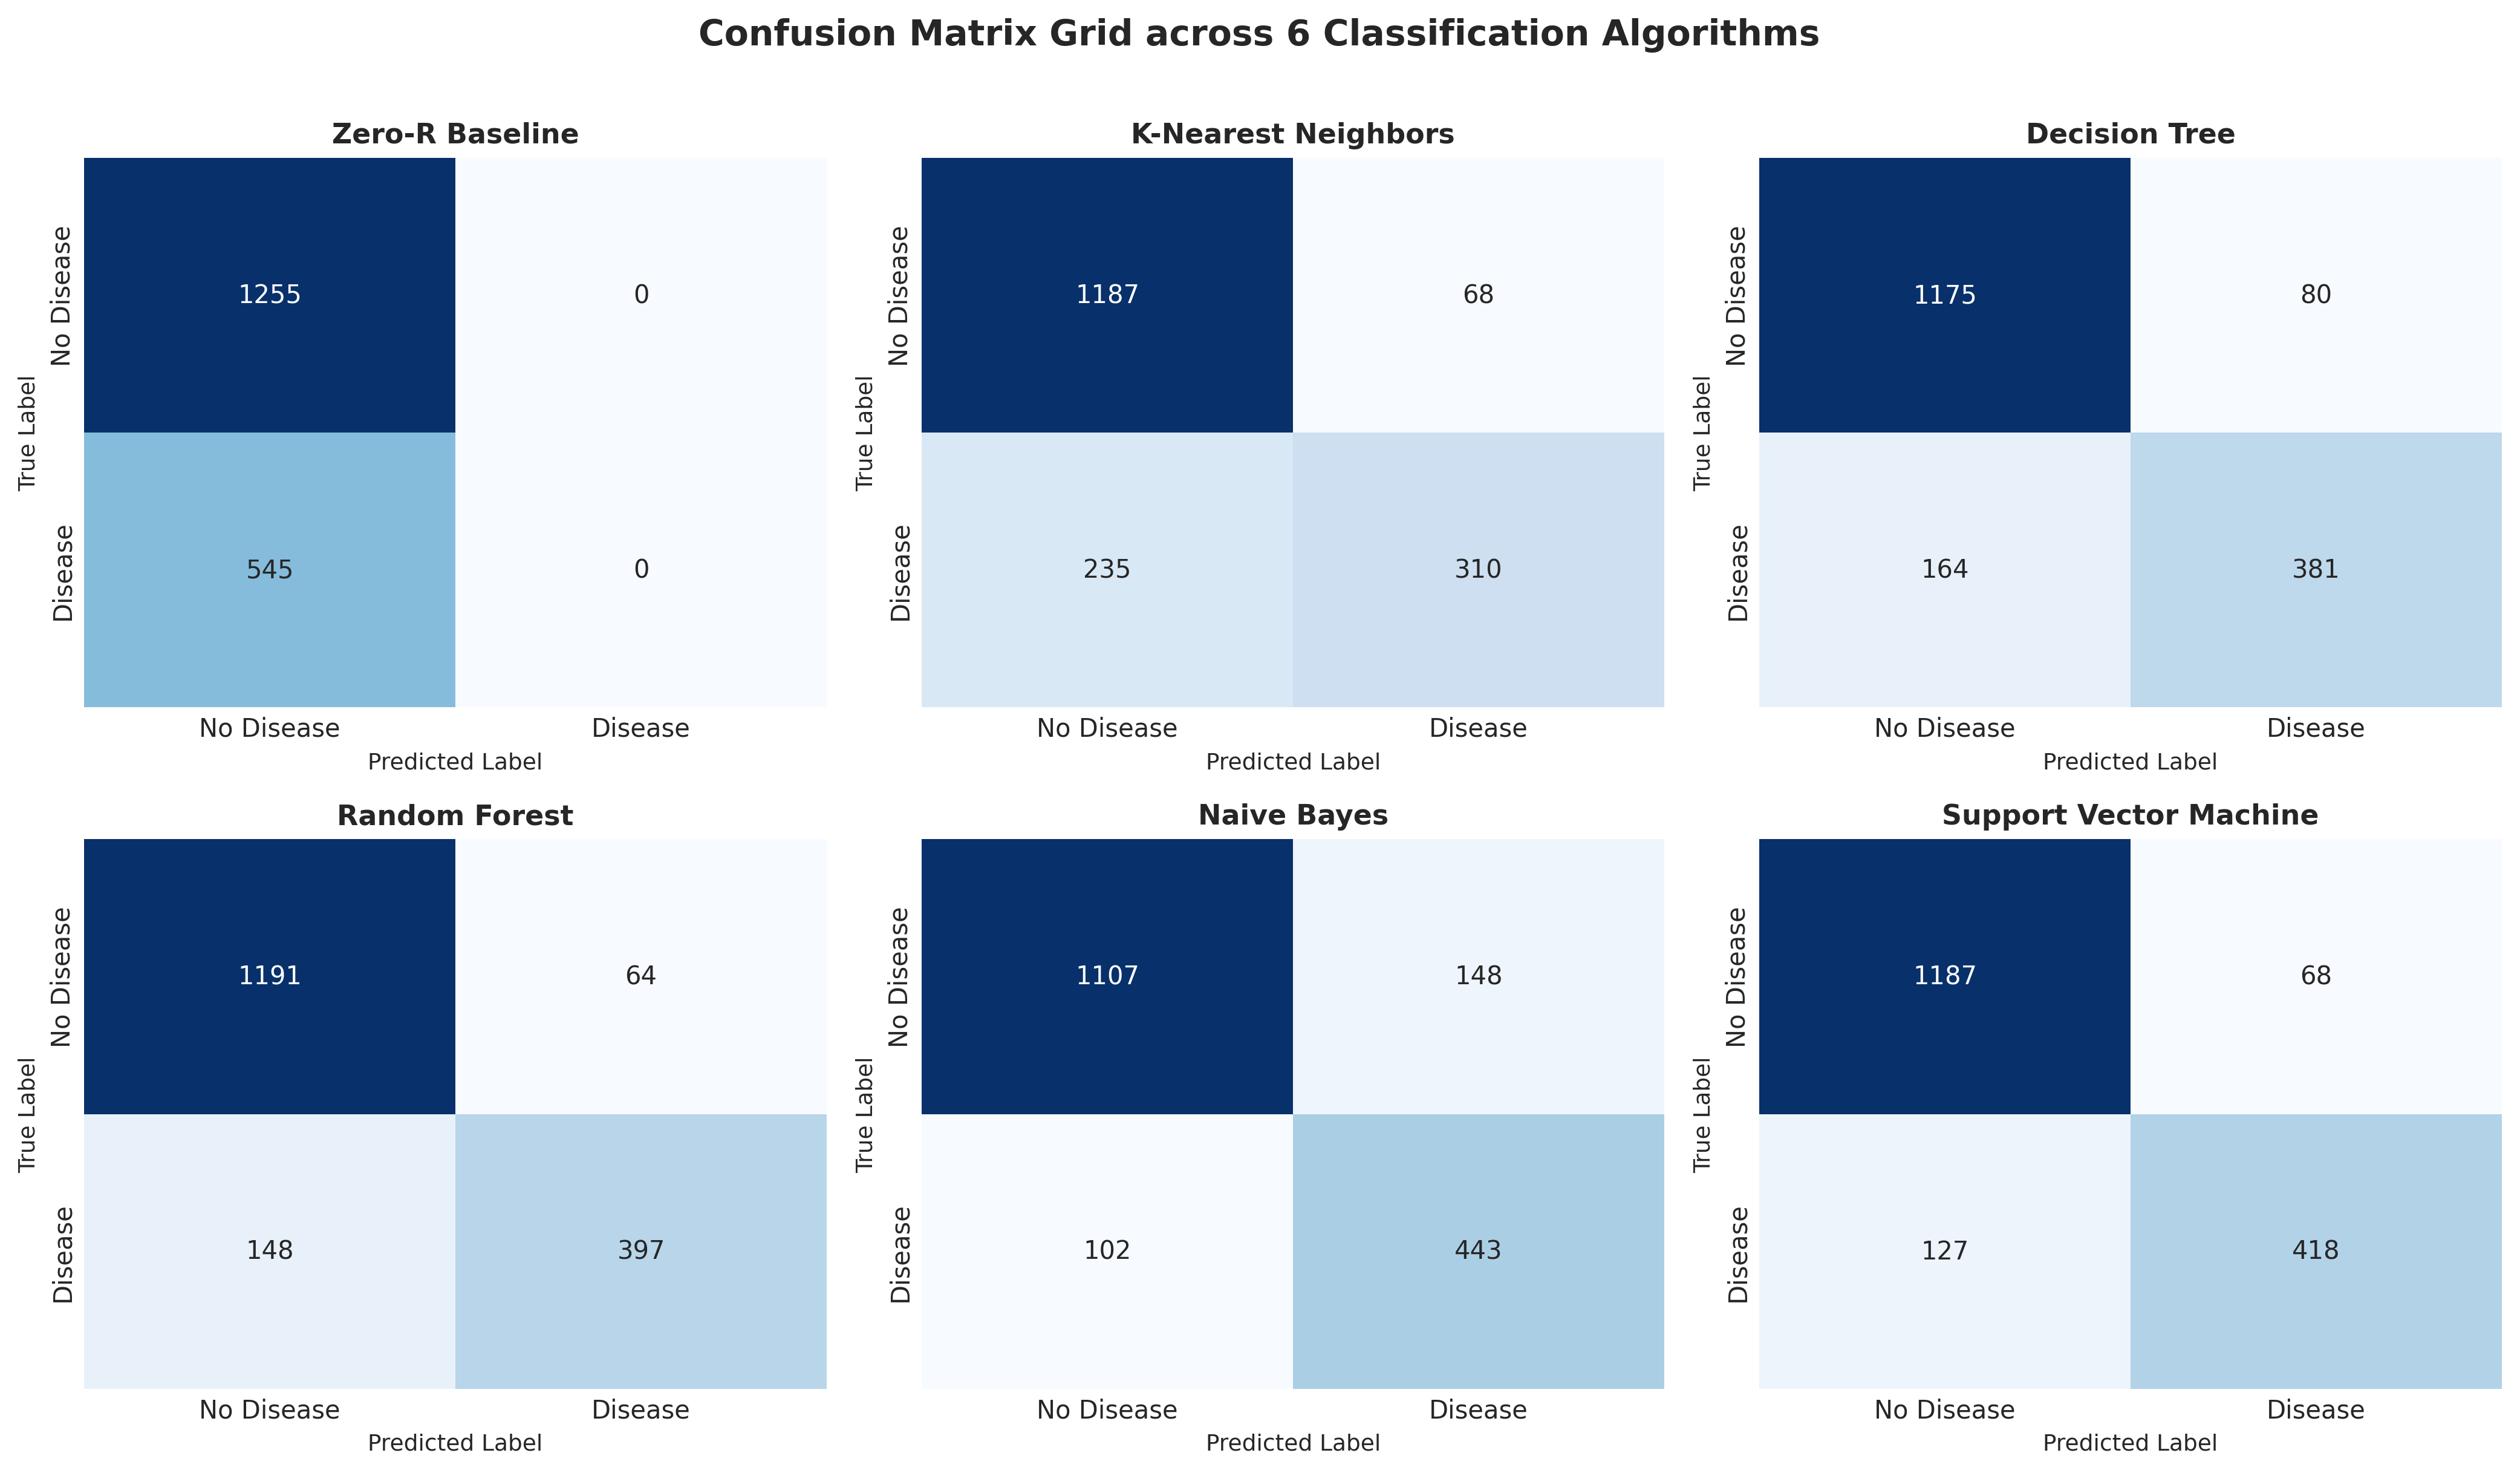
\includegraphics[width=0.8\textwidth]{figures/confusion_matrices.png}
\caption{Confusion Matrix Grid across 6 Classification Algorithms.}
\label{fig:results_cm}
\end{figure}

\subsection{Error Breakdown for Best Classifier (SVM)}
Out of $1,800$ test patients ($1,255$ healthy controls, $545$ diseased patients):
\begin{itemize}
    \item \textbf{True Negatives ($TN$):} $1,187$ healthy patients correctly identified ($94.58\%$ specificity).
    \item \textbf{True Positives ($TP$):} $418$ heart disease patients correctly caught ($76.70\%$ recall).
    \item \textbf{False Positives ($FP$):} $68$ healthy patients misclassified as high risk ($5.42\%$ false alarm rate).
    \item \textbf{False Negatives ($FN$):} $127$ diseased patients misclassified as low risk ($23.30\%$ false negative rate).
\end{itemize}

\section{Multi-Perspective Feature Importance Analysis}
Figure~\ref{fig:results_fi} displays normalized feature importances across four distinct analytical perspectives: Mutual Information, Random Forest Gini Importance, Permutation Importance, and Pearson Correlation Magnitude.

\begin{figure}[H]
\centering
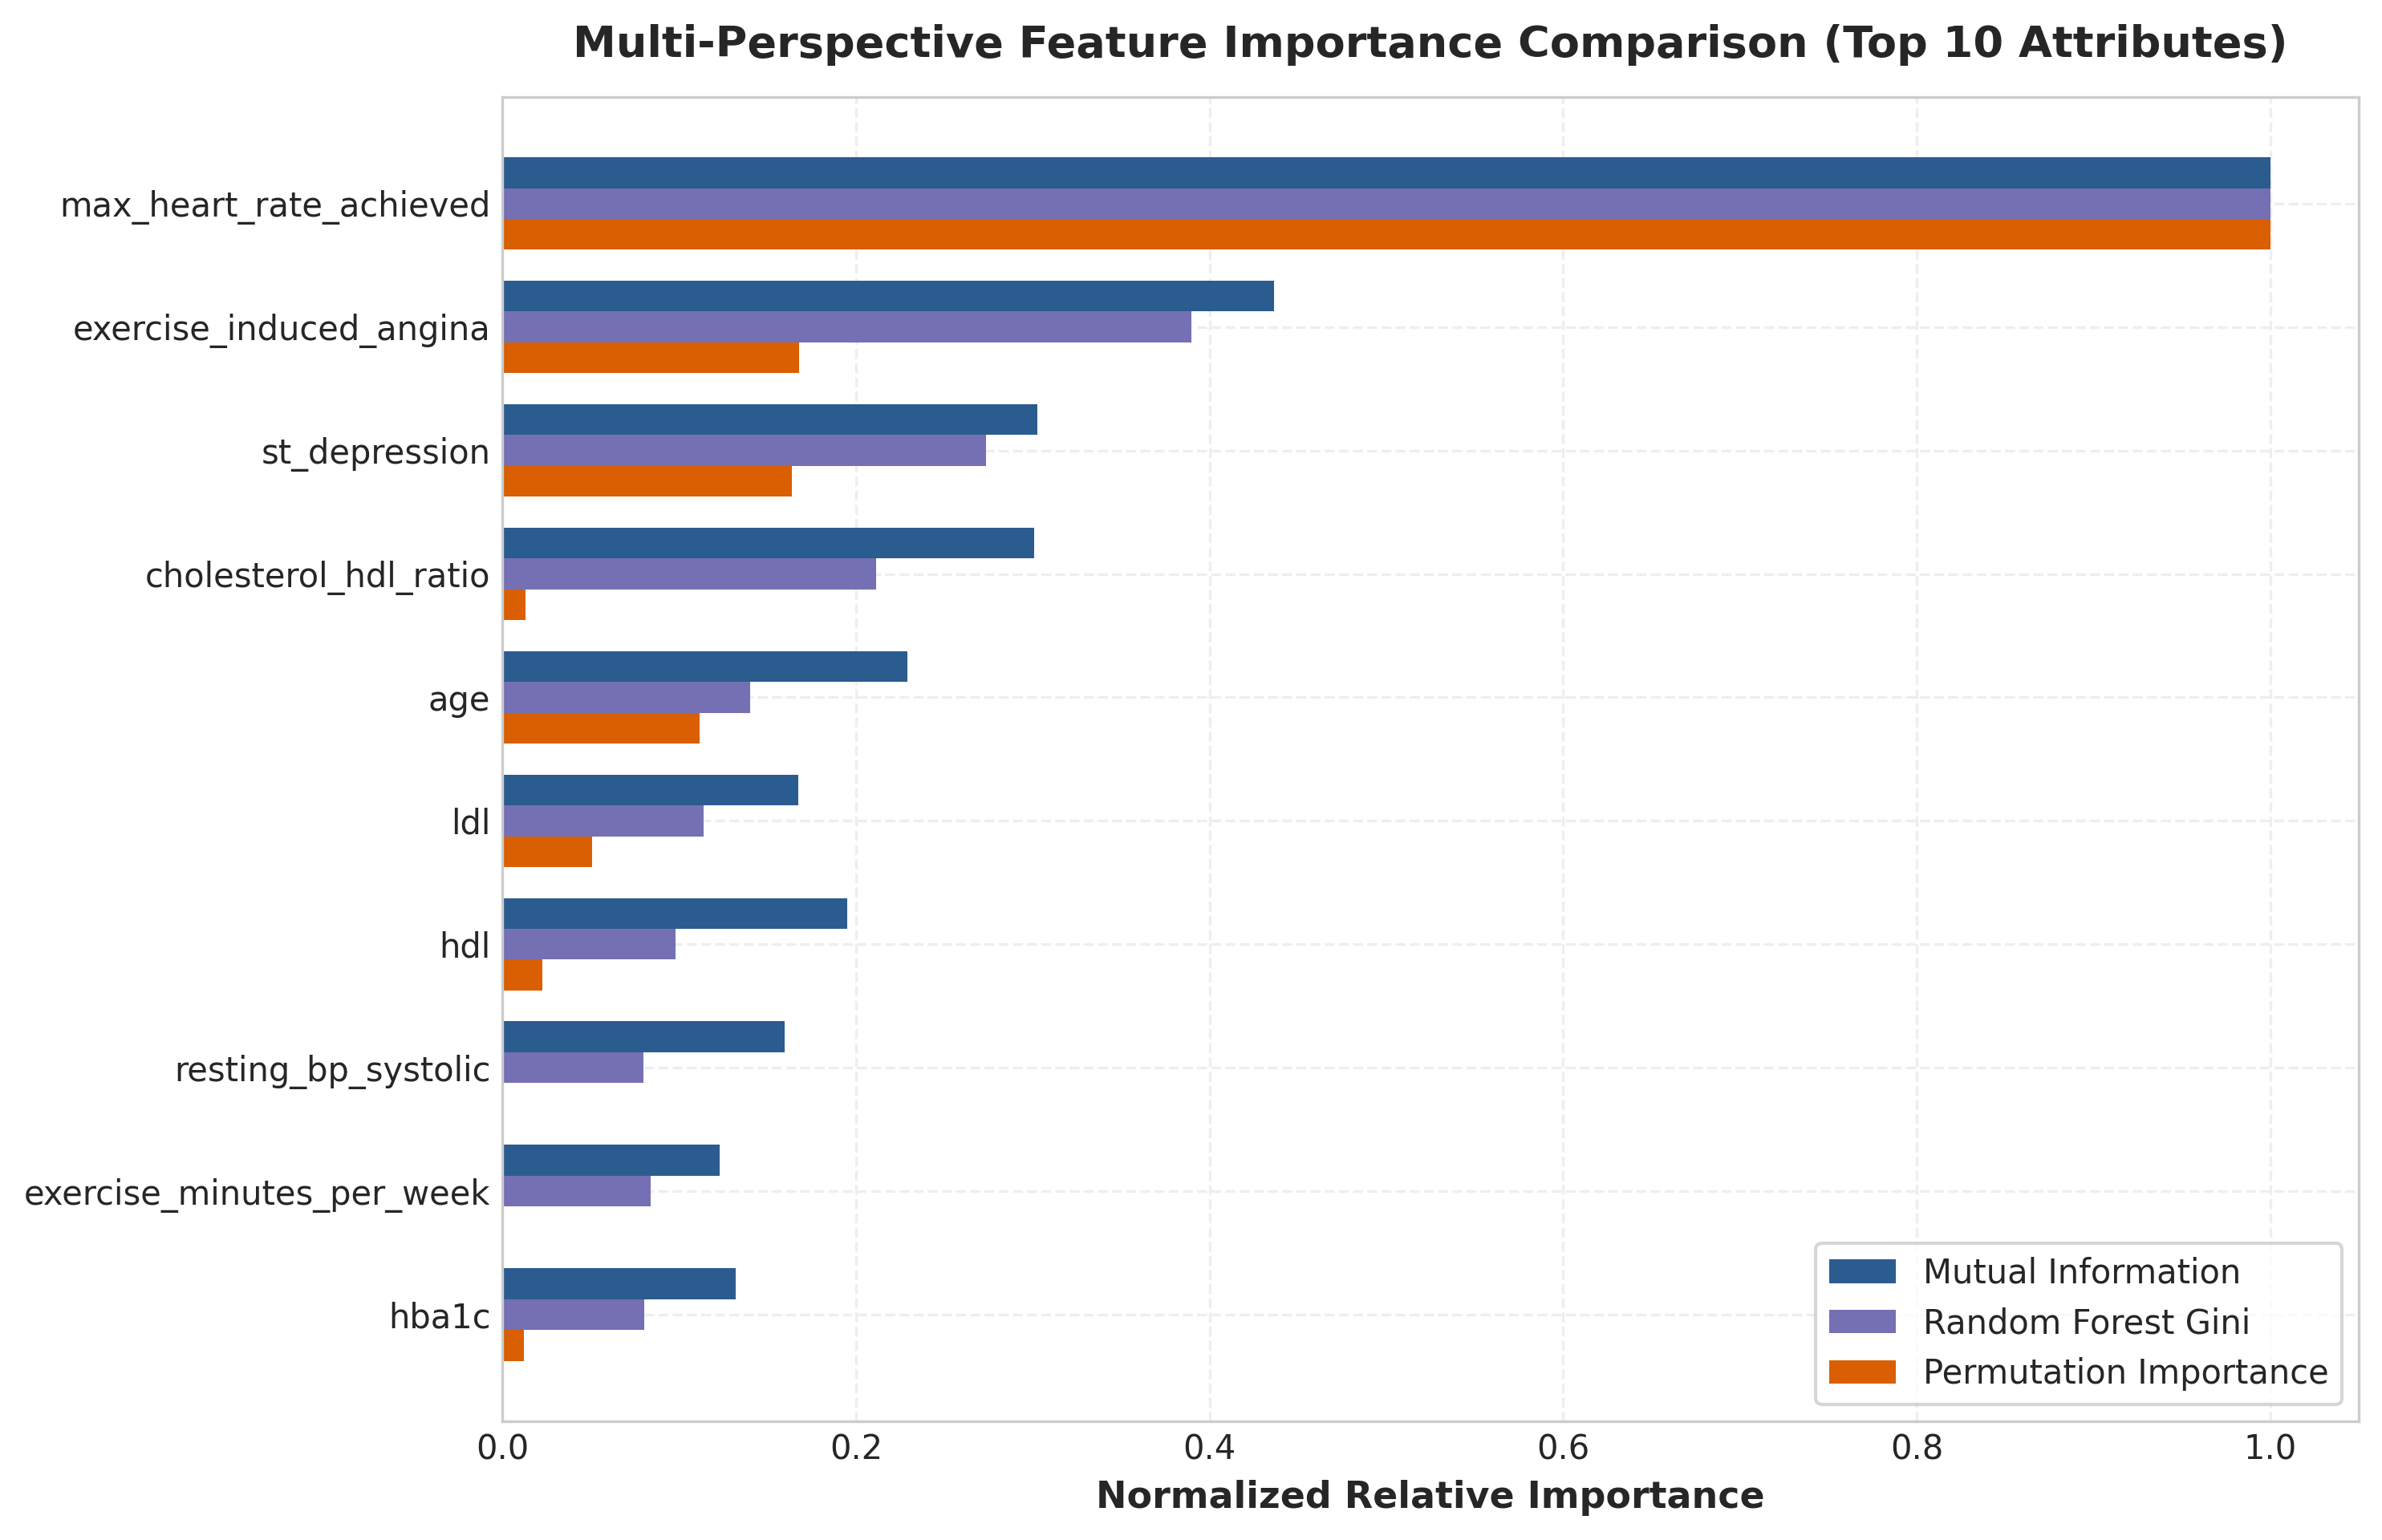
\includegraphics[width=0.8\textwidth]{figures/feature_importance_comp.png}
\caption{Multi-Perspective Feature Importance Comparison.}
\label{fig:results_fi}
\end{figure}

\begin{tcolorbox}[colback=lightbg,colframe=navyblue,title=\textbf{Consensus Top Predictor Cluster}]
\begin{enumerate}
    \item \textbf{Maximum Heart Rate Achieved (\texttt{max\_heart\_rate\_achieved}):} Top negative predictor across all 4 perspectives.
    \item \textbf{ST Segment Depression (\texttt{st\_depression}):} Top positive continuous predictor across all 4 perspectives.
    \item \textbf{Patient Age (\texttt{age}):} Top demographic risk driver.
    \item \textbf{LDL Cholesterol (\texttt{ldl}):} Top blood chemistry biomarker.
\end{enumerate}
\end{tcolorbox}
